\documentclass[11pt,a4paper]{article}
\usepackage[utf8]{inputenc}
\usepackage[T1]{fontenc}
\usepackage{amsmath,amsfonts,amssymb}
\usepackage{graphicx}
\usepackage[margin=1in]{geometry}
\usepackage{listings}
\usepackage{xcolor}
\usepackage{hyperref}
\usepackage{booktabs}
\usepackage{array}
\usepackage{longtable}
\usepackage{float}
\usepackage{enumitem}

% Configure listings for Java code
\lstdefinestyle{javastyle}{
    language=Java,
    backgroundcolor=\color{gray!10},
    basicstyle=\footnotesize\ttfamily,
    keywordstyle=\color{blue}\bfseries,
    commentstyle=\color{green!60!black},
    stringstyle=\color{red},
    numberstyle=\tiny\color{gray},
    stepnumber=1,
    numbersep=5pt,
    frame=single,
    rulecolor=\color{black!30},
    breaklines=true,
    showstringspaces=false,
    tabsize=2
}

% Configure listings for bash
\lstdefinestyle{bashstyle}{
    language=bash,
    backgroundcolor=\color{gray!5},
    basicstyle=\footnotesize\ttfamily,
    keywordstyle=\color{blue}\bfseries,
    commentstyle=\color{green!60!black},
    frame=single,
    rulecolor=\color{black!30},
    breaklines=true,
    showstringspaces=false
}

\lstset{style=javastyle}

\title{Extended Testing Regime for rmatch:\\Comprehensive Performance Validation and Optimization Guidance}
\author{Performance Engineering Proposal}
\date{\today}

\begin{document}

\maketitle

\begin{abstract}
This proposal outlines an extended testing regime for the rmatch regular expression matching library to provide more challenging and diverse test scenarios that enable better assessment of performance improvements and optimization efforts. The current benchmark tests are insufficient for evaluating complex performance characteristics and guiding optimization decisions. We propose a comprehensive suite of test scenarios, metrics, and evaluation frameworks that will provide clearer insights into performance bottlenecks and optimization opportunities.
\end{abstract}

\tableofcontents
\newpage

\section{Executive Summary}

The rmatch library currently lacks comprehensive testing scenarios that can effectively guide performance optimization efforts. The existing benchmarks, while functional, do not provide sufficient diversity in test cases to reveal performance characteristics across different usage patterns, pattern complexities, and input characteristics.

This proposal presents:
\begin{itemize}
    \item A comprehensive taxonomy of test scenarios covering diverse regex patterns and input characteristics
    \item Advanced performance metrics beyond simple throughput measurements
    \item Automated test generation and validation frameworks
    \item Integration with existing CI/CD pipelines for continuous performance monitoring
    \item Clear guidance for interpreting results and prioritizing optimization efforts
\end{itemize}

\section{Problem Analysis}

\subsection{Current Testing Limitations}

The existing benchmark infrastructure has several limitations that hinder effective performance optimization:

\begin{enumerate}
    \item \textbf{Limited Pattern Diversity}: Current tests focus primarily on simple word-matching patterns from literary text
    \item \textbf{Insufficient Input Variety}: Testing is concentrated on a single corpus (Wuthering Heights)
    \item \textbf{Basic Metrics}: Performance evaluation relies mainly on throughput and memory usage
    \item \textbf{No Stress Testing}: Lack of tests for edge cases, pathological patterns, or extreme scale scenarios
    \item \textbf{Missing Regression Detection}: No systematic approach to detect performance regressions across different optimization approaches
\end{enumerate}

\subsection{Impact on Optimization Efforts}

These limitations create several challenges for performance optimization:

\begin{itemize}
    \item Difficulty in identifying which optimizations provide real-world benefits
    \item Risk of optimizing for narrow use cases while degrading performance elsewhere
    \item Inability to validate optimization effectiveness across diverse scenarios
    \item Lack of confidence in performance improvements due to limited test coverage
\end{itemize}

\section{Proposed Testing Framework}

\subsection{Test Categories}

We propose organizing tests into several categories that cover different aspects of performance:

\subsubsection{Pattern Complexity Tests}

\begin{figure}[H]
\centering
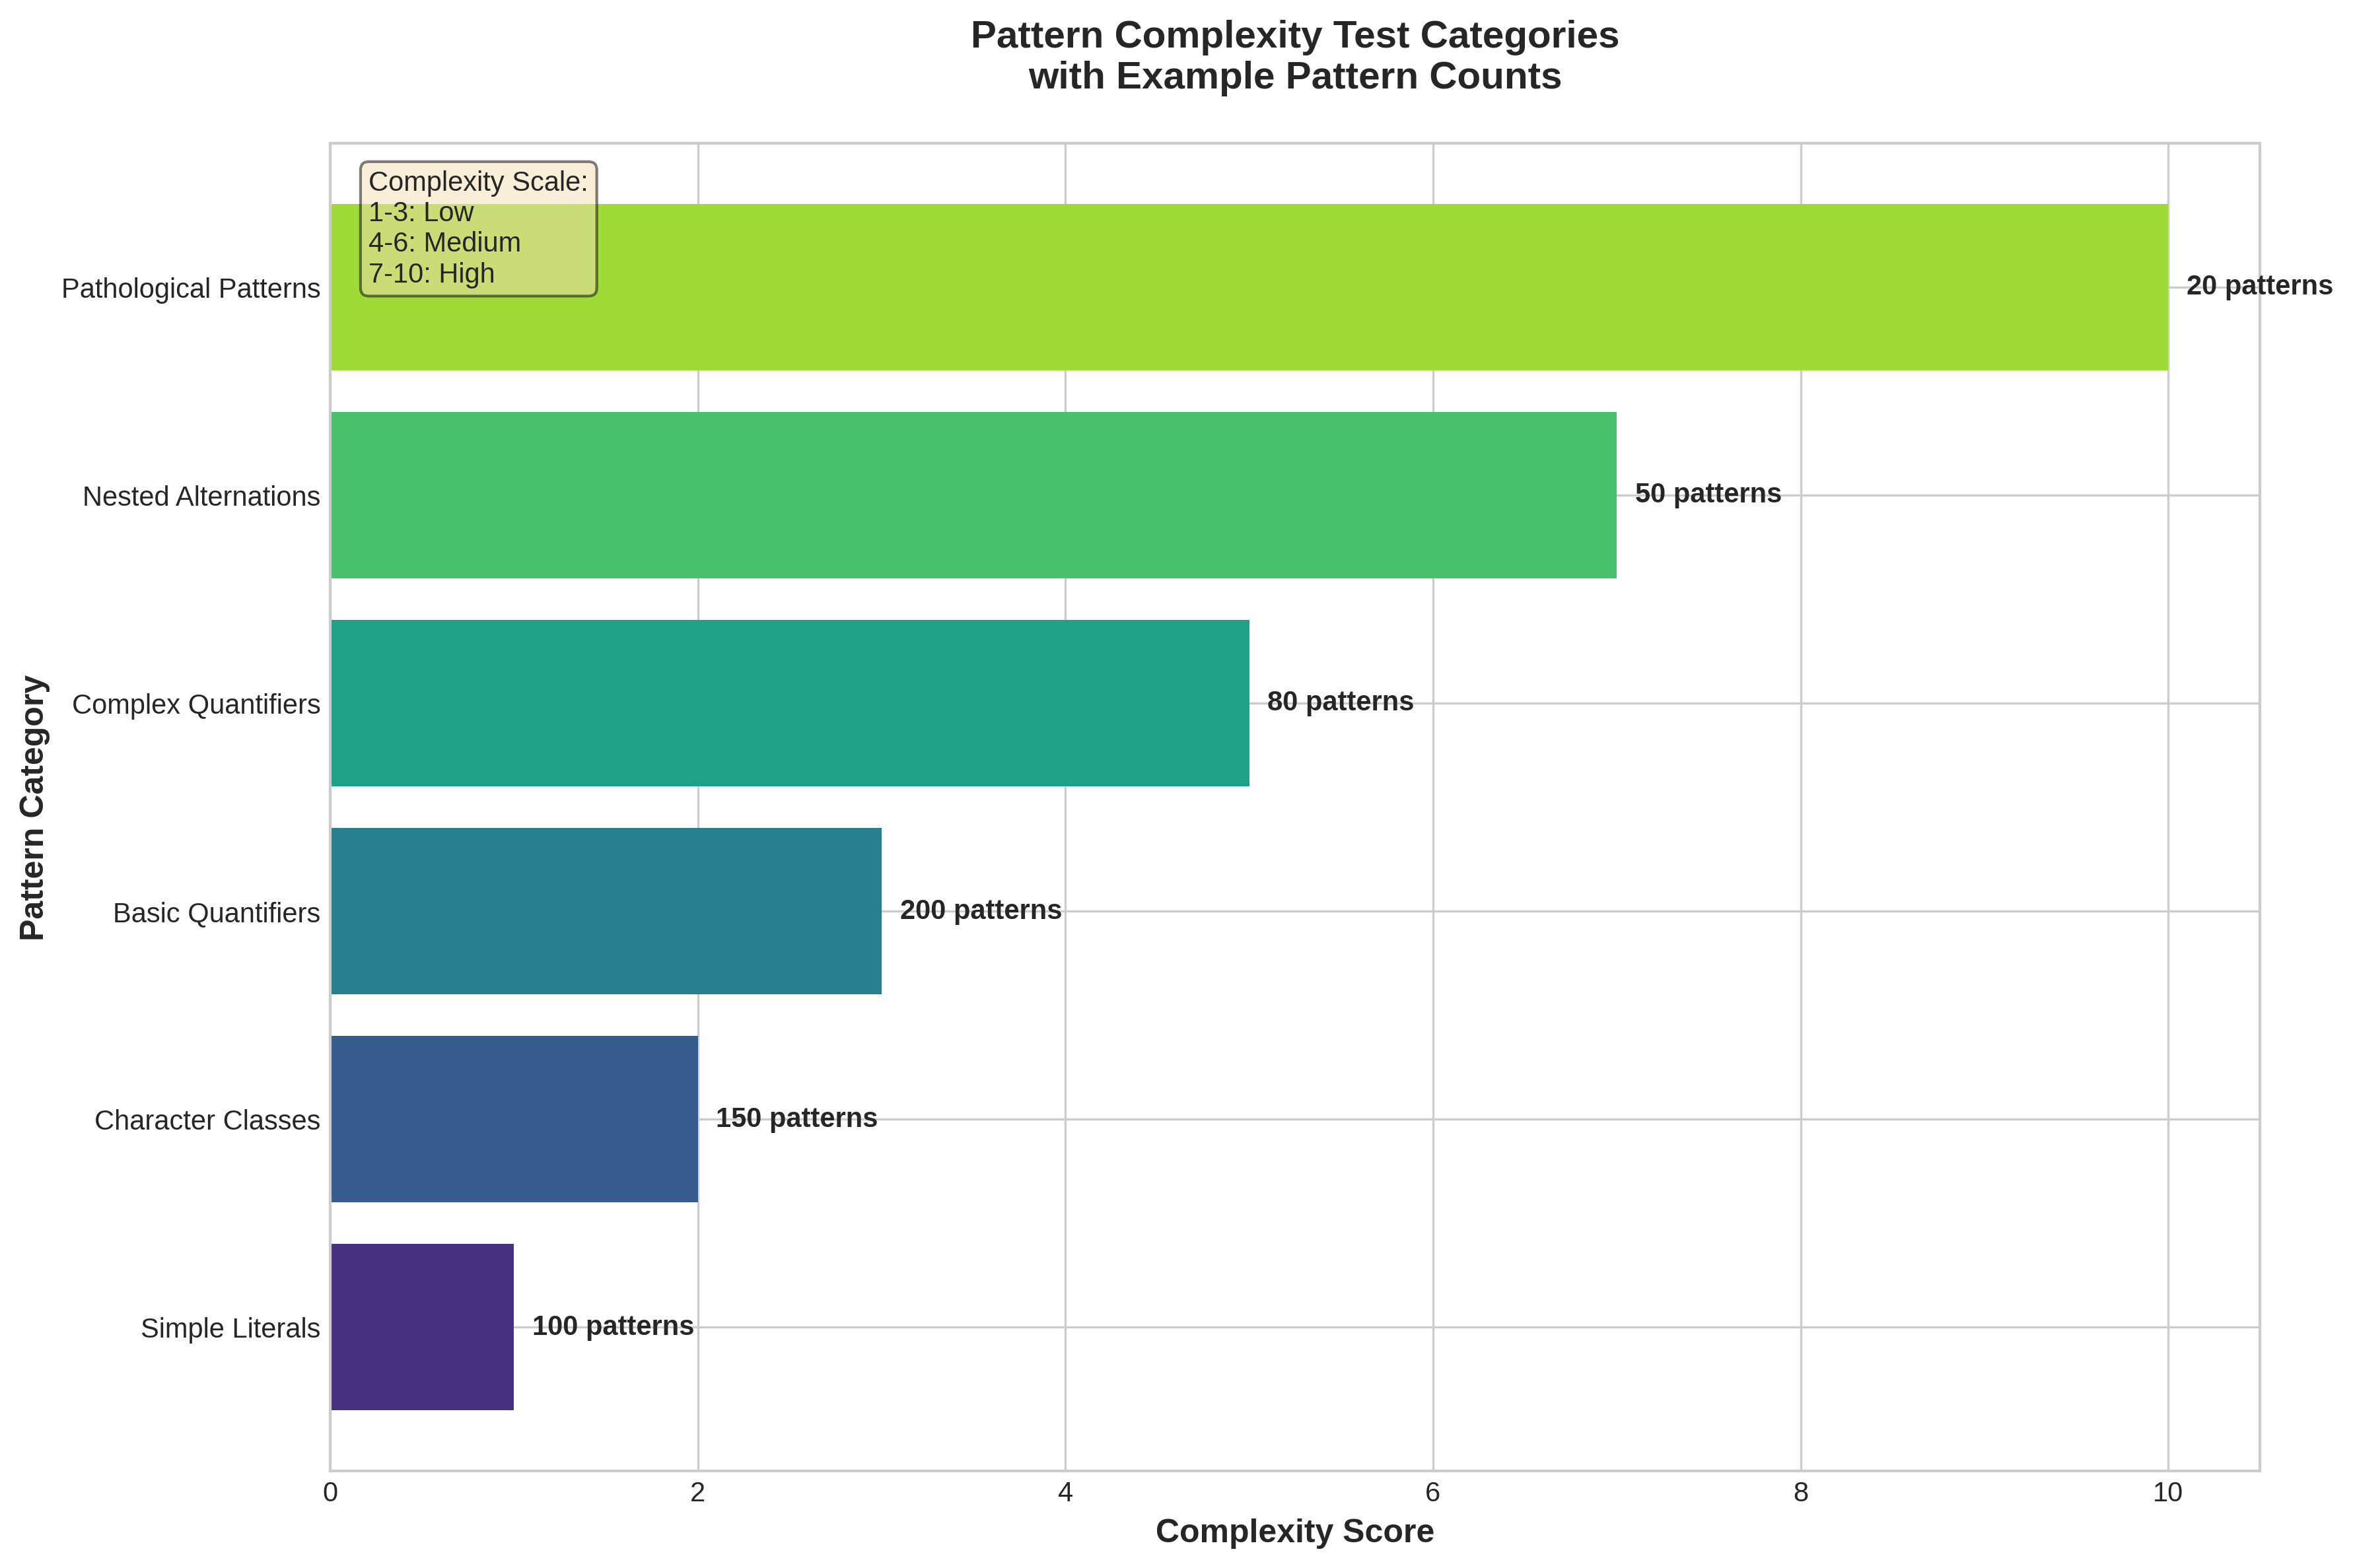
\includegraphics[width=0.8\textwidth]{illustrations/pattern_complexity_taxonomy.png}
\caption{Pattern Complexity Test Categories}
\label{fig:pattern_complexity}
\end{figure}

\begin{enumerate}
    \item \textbf{Simple Literal Patterns}: Basic string matching scenarios
    \item \textbf{Character Class Patterns}: Testing various character class implementations
    \item \textbf{Quantifier Stress Tests}: Patterns with complex quantifier combinations
    \item \textbf{Alternation Complexity}: Nested and complex alternation patterns
    \item \textbf{Pathological Patterns}: Known problematic patterns for regex engines
\end{enumerate}

\subsubsection{Input Characteristic Tests}

\begin{figure}[H]
\centering
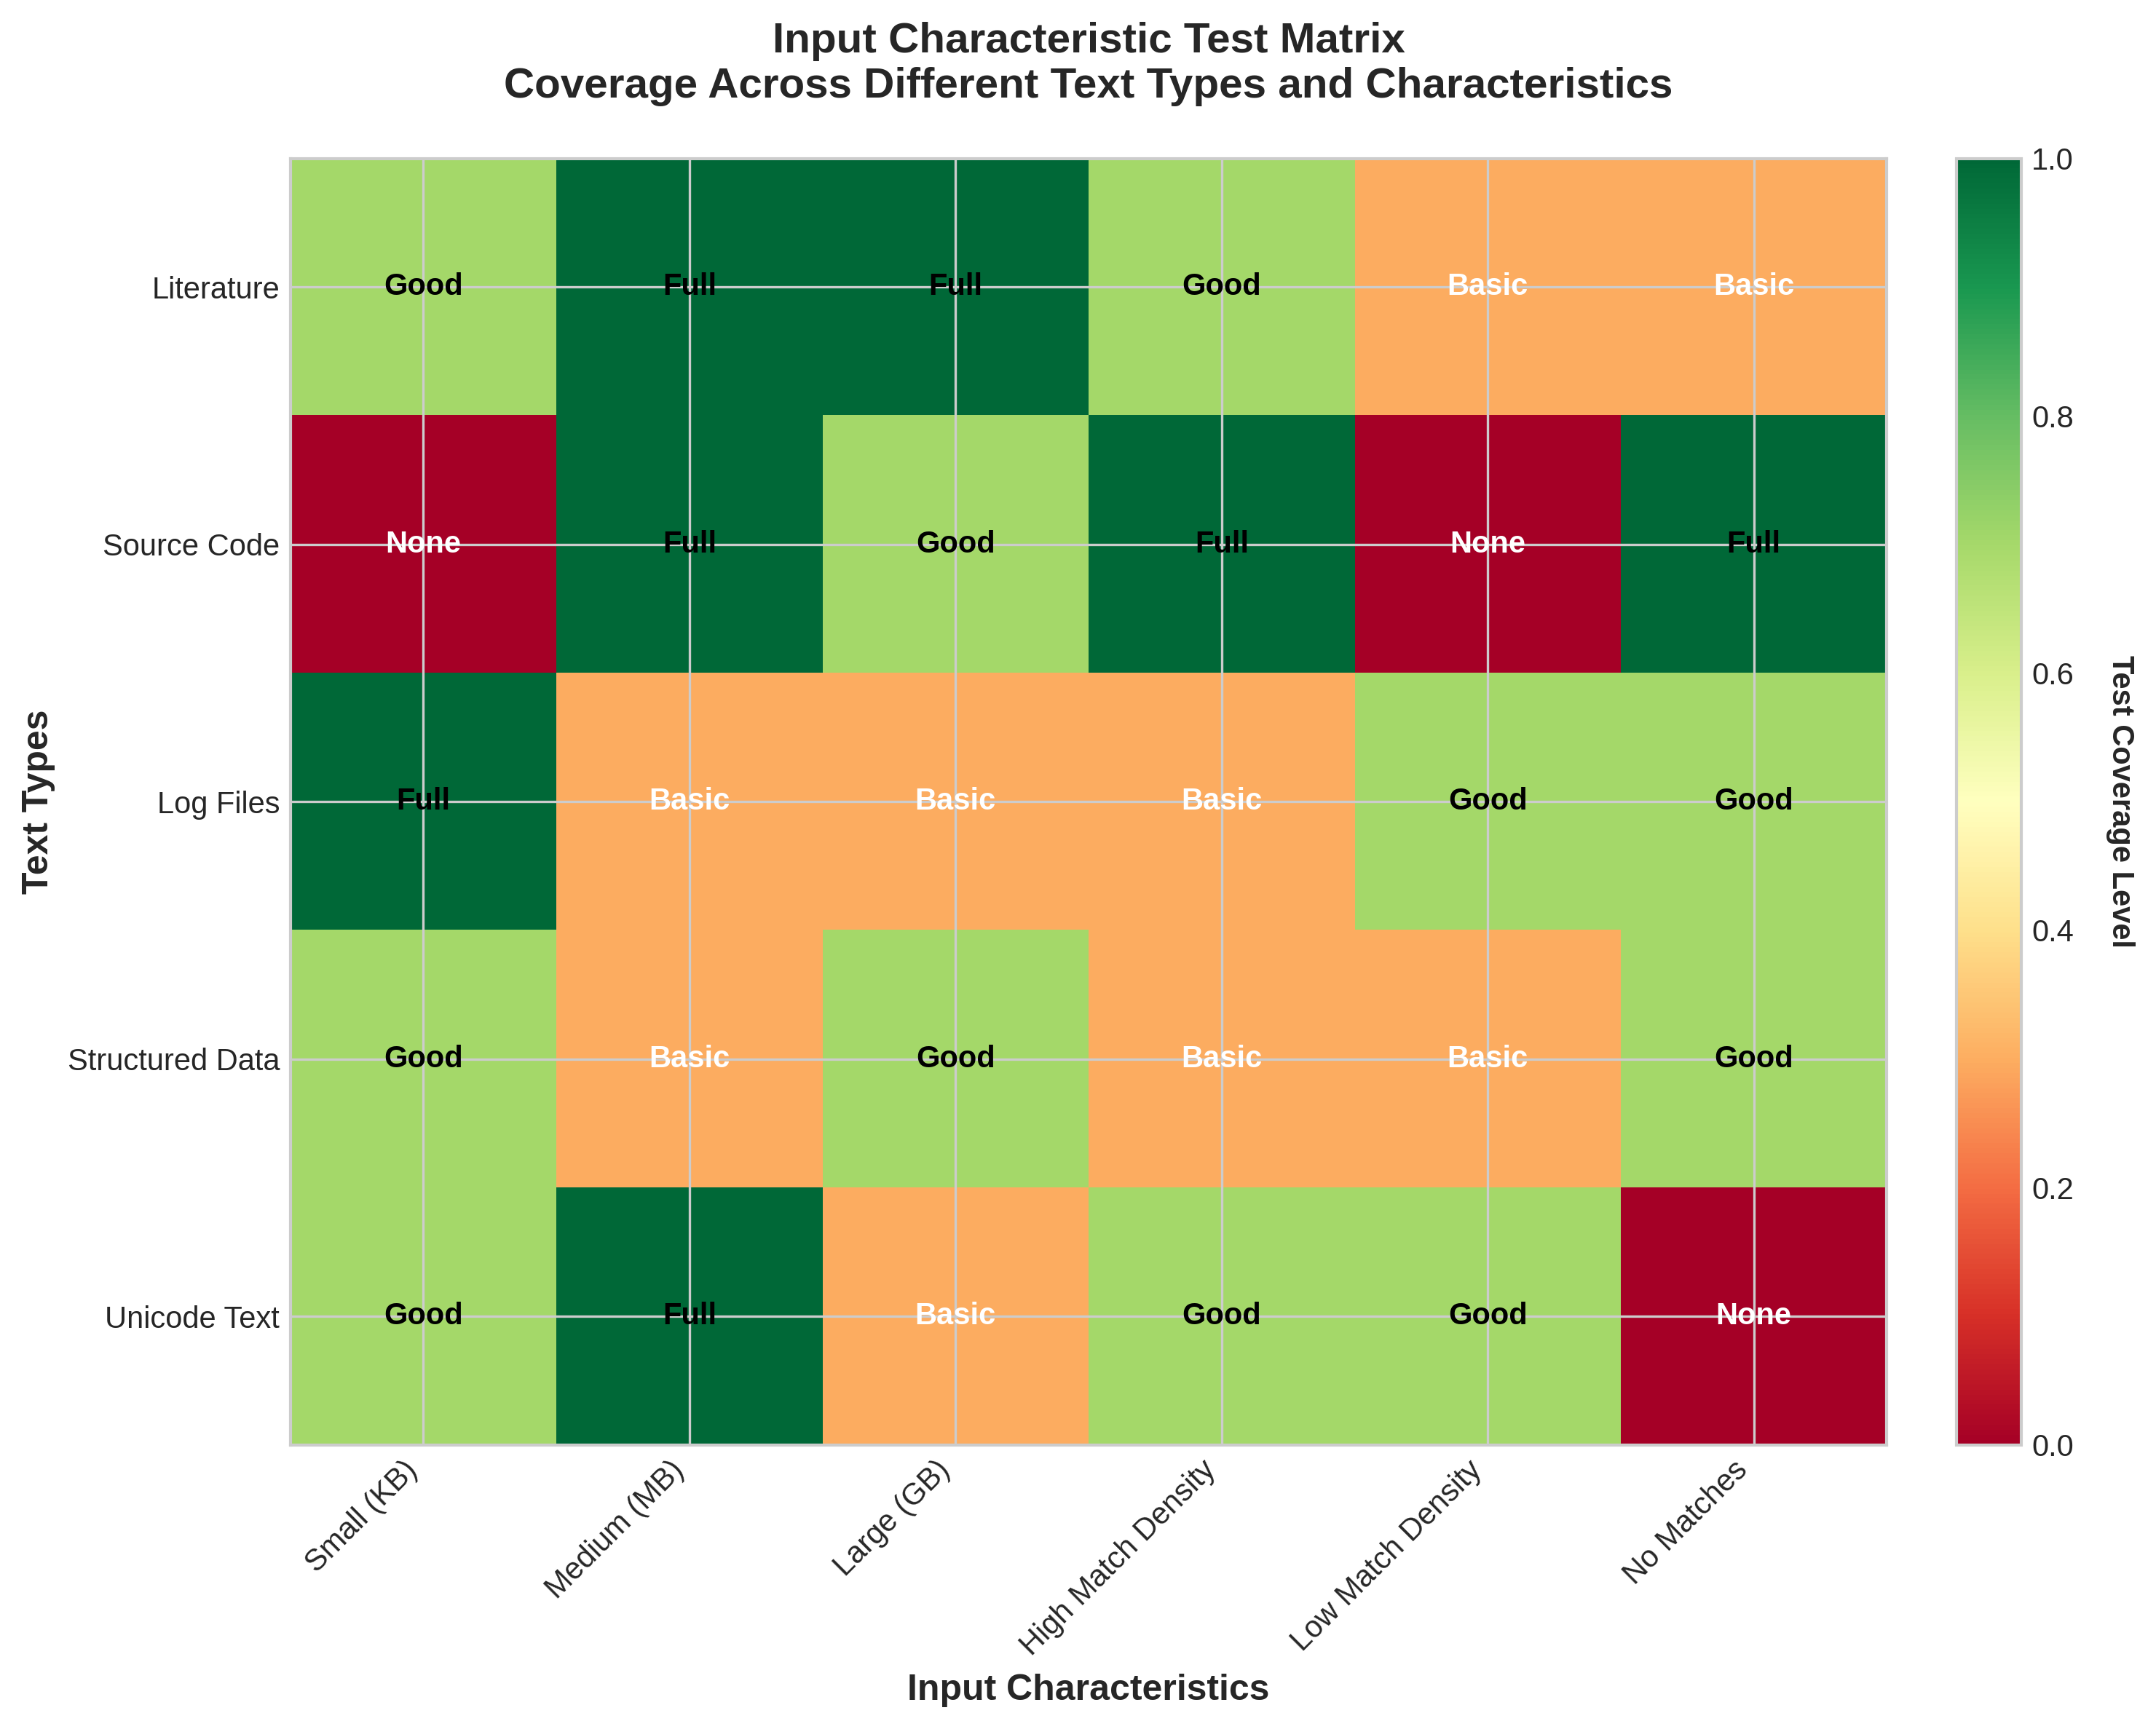
\includegraphics[width=0.8\textwidth]{illustrations/input_characteristics.png}
\caption{Input Characteristic Test Matrix}
\label{fig:input_characteristics}
\end{figure}

\begin{enumerate}
    \item \textbf{Text Structure Variation}: Different text types (code, natural language, structured data)
    \item \textbf{Match Density Scenarios}: High-match, low-match, and no-match scenarios
    \item \textbf{Input Size Scaling}: Testing performance across different input sizes
    \item \textbf{Unicode Complexity}: Various Unicode character sets and normalization scenarios
\end{enumerate}

\subsubsection{Scale and Concurrency Tests}

\begin{enumerate}
    \item \textbf{Pattern Set Size Scaling}: Testing with 1 to 100,000+ patterns
    \item \textbf{Concurrent Matching}: Multi-threaded performance characteristics
    \item \textbf{Memory Pressure Tests}: Performance under various memory constraints
    \item \textbf{Long-Running Scenarios}: Sustained performance over extended periods
\end{enumerate}

\subsection{Advanced Metrics Framework}

Beyond basic throughput and memory usage, we propose collecting detailed performance metrics:

\begin{table}[H]
\centering
\begin{tabular}{@{}lp{8cm}@{}}
\toprule
\textbf{Metric Category} & \textbf{Specific Metrics} \\
\midrule
Throughput & MB/s, patterns/s, matches/s, characters/s \\
Latency & P50, P95, P99 response times, worst-case latency \\
Memory & Peak usage, allocation rate, GC pressure, memory efficiency \\
CPU & CPU utilization, cache miss rates, instruction throughput \\
Scalability & Throughput vs. pattern count, memory vs. pattern count \\
Quality & Match accuracy, false positive/negative rates \\
\bottomrule
\end{tabular}
\caption{Comprehensive Performance Metrics}
\label{tab:metrics}
\end{table}

\subsection{Test Data Generation}

\begin{figure}[H]
\centering
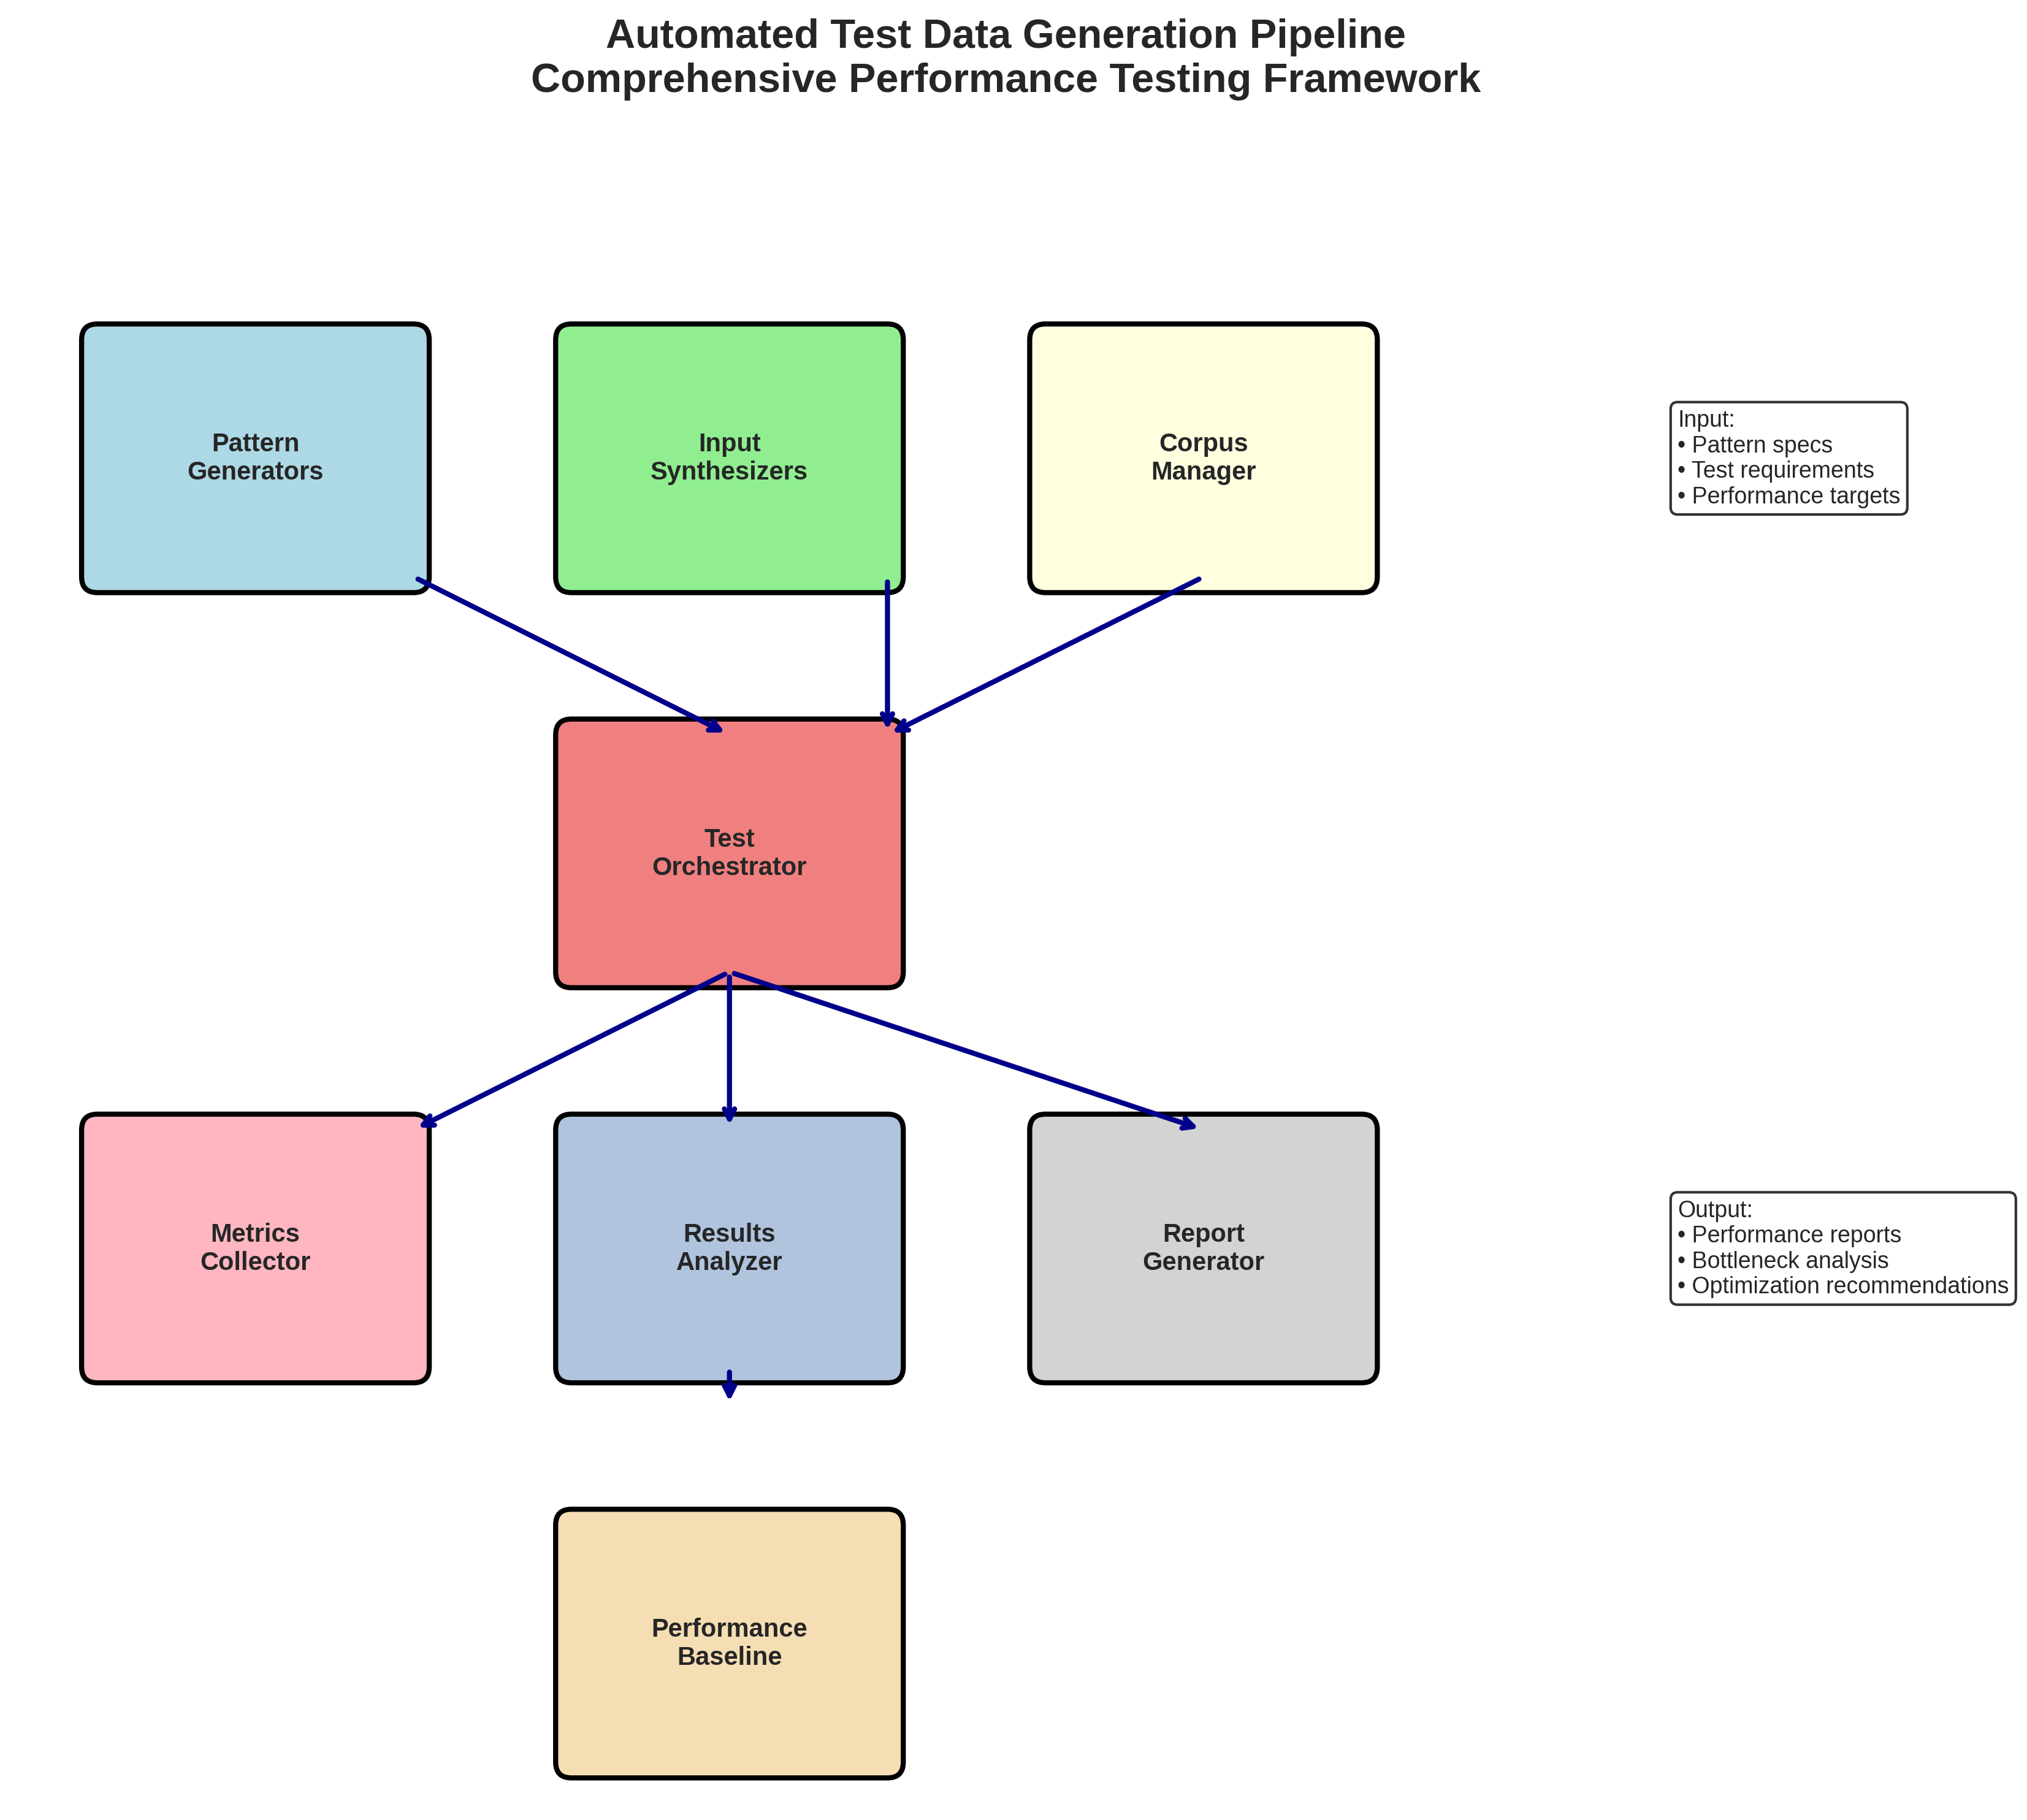
\includegraphics[width=0.9\textwidth]{illustrations/test_generation_pipeline.png}
\caption{Automated Test Data Generation Pipeline}
\label{fig:test_generation}
\end{figure}

We propose an automated test generation system that creates diverse test scenarios:

\begin{enumerate}
    \item \textbf{Pattern Generators}: Algorithmic generation of patterns with specific characteristics
    \item \textbf{Input Synthesizers}: Creation of synthetic inputs that stress different aspects of the engine
    \item \textbf{Corpus Diversification}: Automatic expansion of test corpora from various domains
    \item \textbf{Property-Based Testing}: Randomized testing with invariant checking
\end{enumerate}

\section{Implementation Architecture}

\subsection{Framework Components}

\begin{figure}[H]
\centering
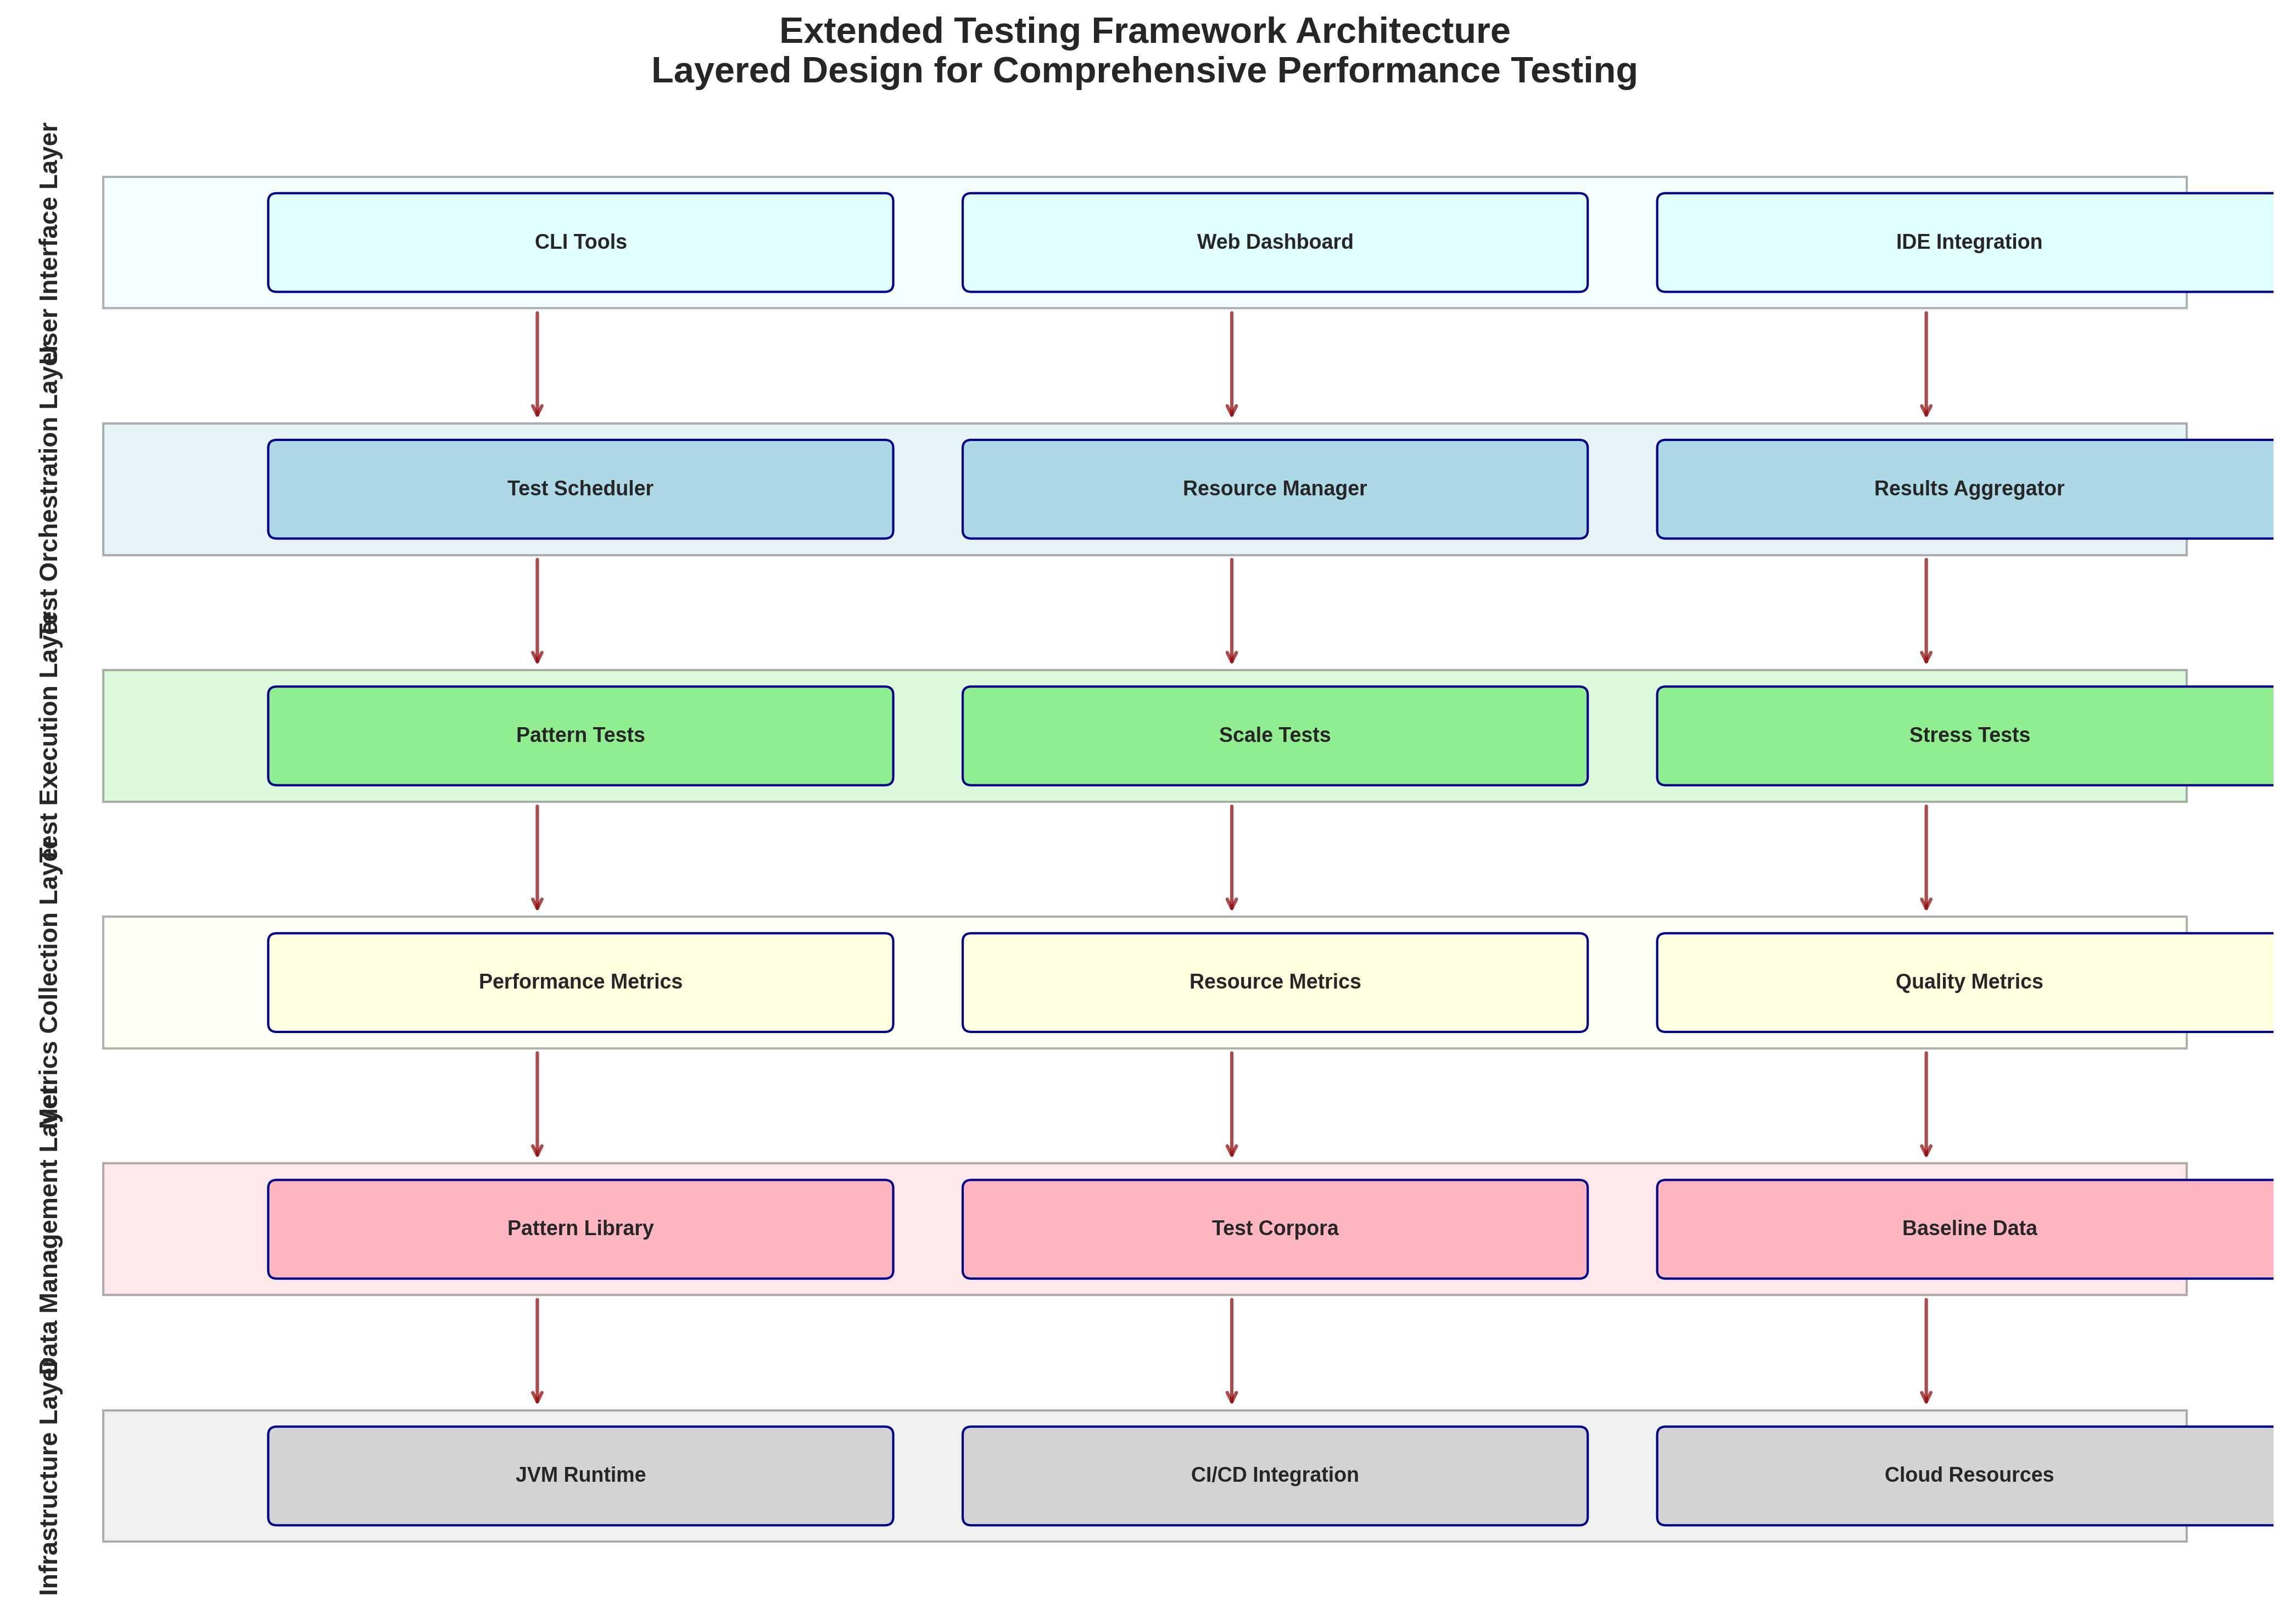
\includegraphics[width=0.9\textwidth]{illustrations/testing_architecture.png}
\caption{Extended Testing Framework Architecture}
\label{fig:architecture}
\end{figure}

The testing framework consists of several interconnected components:

\begin{enumerate}
    \item \textbf{Test Orchestrator}: Coordinates test execution and result collection
    \item \textbf{Pattern Library}: Curated collection of test patterns organized by category
    \item \textbf{Corpus Manager}: Manages diverse test input corpora
    \item \textbf{Metrics Collector}: Gathers comprehensive performance metrics
    \item \textbf{Results Analyzer}: Processes and interprets test results
    \item \textbf{Report Generator}: Creates actionable performance reports
\end{enumerate}

\subsection{Integration with Existing Infrastructure}

The extended testing framework integrates seamlessly with existing rmatch infrastructure:

\begin{itemize}
    \item Extends existing JMH benchmarks with new test scenarios
    \item Integrates with GitHub Actions for continuous performance monitoring
    \item Maintains compatibility with existing baseline management
    \item Provides migration path from current testing approaches
\end{itemize}

\section{Performance Insights and Optimization Guidance}

\subsection{Performance Characterization}

The extended testing regime will provide insights into:

\begin{figure}[H]
\centering
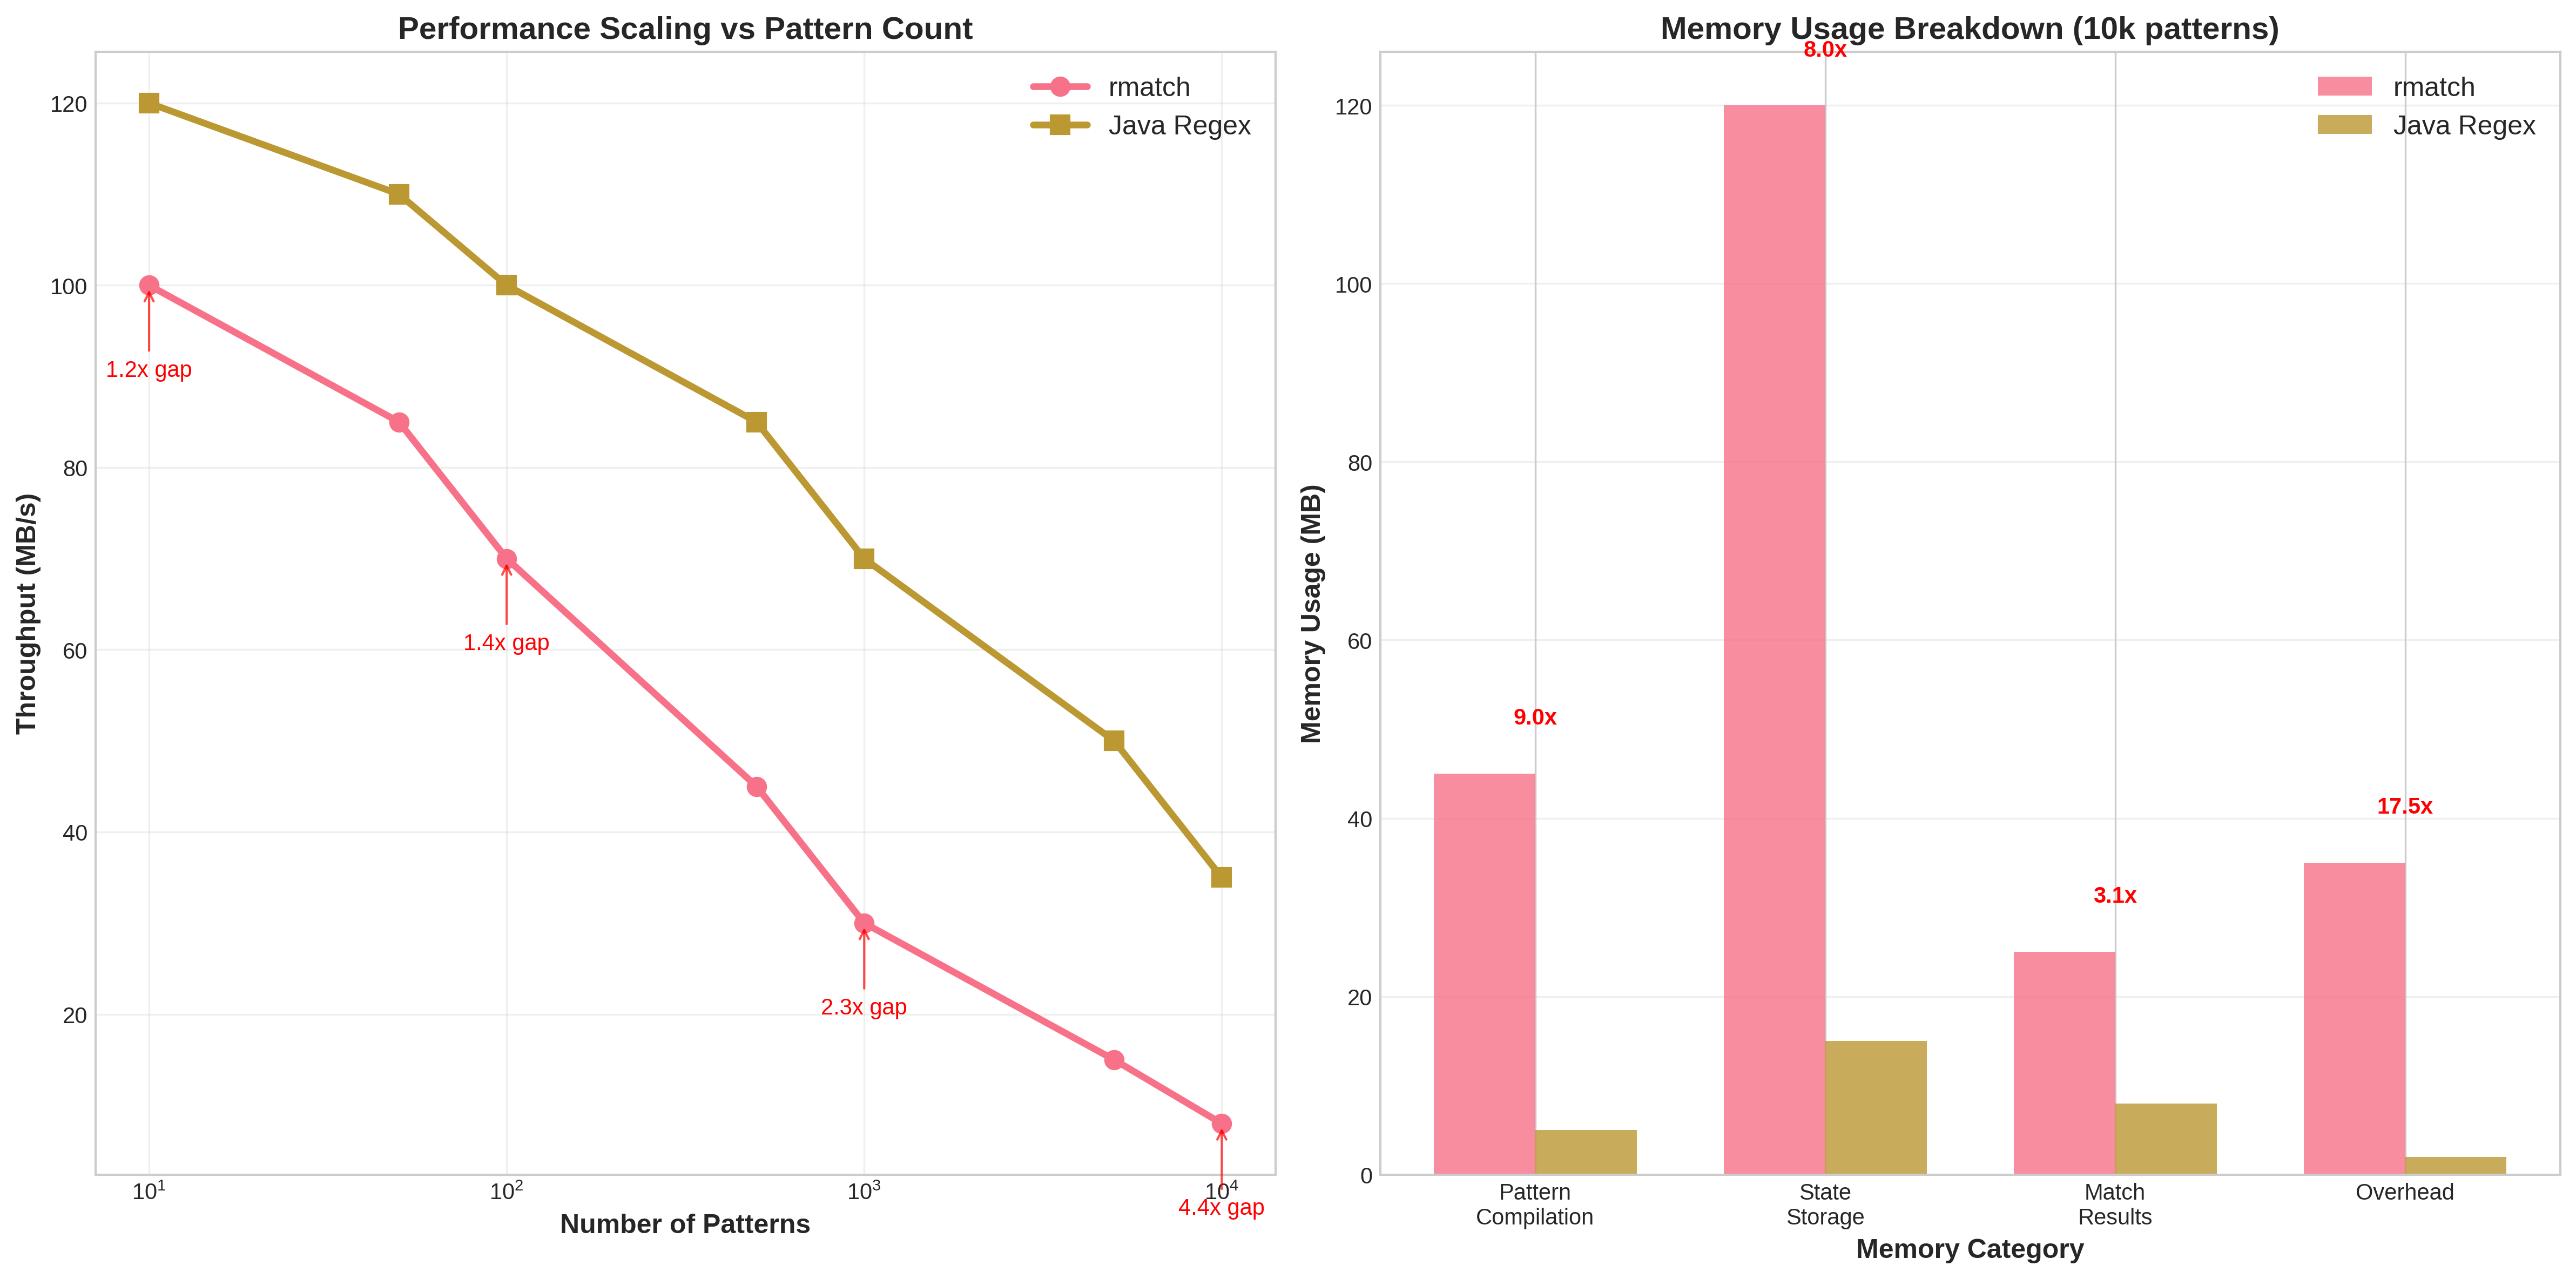
\includegraphics[width=0.8\textwidth]{illustrations/performance_characterization.png}
\caption{Performance Characterization Matrix}
\label{fig:performance_char}
\end{figure}

\begin{enumerate}
    \item \textbf{Algorithmic Complexity}: How performance scales with input and pattern complexity
    \item \textbf{Implementation Bottlenecks}: Specific code paths that limit performance
    \item \textbf{Resource Utilization}: Efficiency of CPU, memory, and cache usage
    \item \textbf{Trade-off Analysis}: Performance vs. memory vs. compilation time trade-offs
\end{enumerate}

\subsection{Optimization Prioritization}

Results from the extended testing will guide optimization efforts by:

\begin{itemize}
    \item Identifying scenarios where rmatch underperforms most significantly
    \item Revealing optimization opportunities with the highest impact potential
    \item Providing clear metrics for measuring optimization effectiveness
    \item Enabling data-driven decision making for algorithmic improvements
\end{itemize}

\section{Expected Benefits}

\subsection{Short-term Benefits}

\begin{itemize}
    \item Clear identification of current performance bottlenecks
    \item Validation of existing optimization hypotheses
    \item Improved confidence in performance claims
    \item Better understanding of competitive positioning vs. Java regex
\end{itemize}

\subsection{Long-term Benefits}

\begin{itemize}
    \item Systematic approach to performance optimization
    \item Reduced risk of performance regressions
    \item Enhanced ability to evaluate new algorithmic approaches
    \item Foundation for performance-driven development processes
\end{itemize}

\section{Implementation Timeline}

\begin{table}[H]
\centering
\begin{tabular}{@{}llp{6cm}@{}}
\toprule
\textbf{Phase} & \textbf{Duration} & \textbf{Deliverables} \\
\midrule
Phase 1 & 2-3 weeks & Test framework foundation, basic pattern library \\
Phase 2 & 3-4 weeks & Advanced metrics collection, test generation \\
Phase 3 & 2-3 weeks & CI/CD integration, automated reporting \\
Phase 4 & 2-3 weeks & Documentation, optimization guidance \\
\midrule
\textbf{Total} & \textbf{9-13 weeks} & \textbf{Complete extended testing regime} \\
\bottomrule
\end{tabular}
\caption{Implementation Timeline}
\label{tab:timeline}
\end{table}

\section{Risk Mitigation}

\subsection{Technical Risks}

\begin{itemize}
    \item \textbf{Test Execution Time}: Mitigate with parallel execution and test prioritization
    \item \textbf{Result Interpretation Complexity}: Provide clear guidelines and automated analysis
    \item \textbf{Maintenance Overhead}: Design for modularity and automated maintenance
\end{itemize}

\subsection{Organizational Risks}

\begin{itemize}
    \item \textbf{Resource Requirements}: Implement incrementally to manage resource usage
    \item \textbf{Adoption Resistance}: Provide clear value demonstration and migration support
    \item \textbf{Tool Complexity}: Ensure user-friendly interfaces and comprehensive documentation
\end{itemize}

\section{Conclusion}

The proposed extended testing regime addresses critical limitations in the current rmatch testing infrastructure. By providing comprehensive, diverse, and automated testing scenarios, it will enable more effective performance optimization and provide clearer guidance for development priorities.

The framework's modular design ensures compatibility with existing infrastructure while providing a foundation for systematic performance improvement efforts. Implementation can proceed incrementally, providing immediate value while building toward the complete testing regime.

\appendix

\section{Task Implementation Guide}

This appendix provides detailed task descriptions for implementing the extended testing regime through the GitHub agent. Each task is designed to be self-contained and executable in sequence.

\subsection{Task 001: Foundation Infrastructure}

\subsubsection{Title}
Set up Extended Testing Framework Foundation

\subsubsection{Problem}
The current testing infrastructure lacks the foundation for comprehensive performance testing. We need to establish the basic framework components that will support advanced testing scenarios.

\subsubsection{Proposal}
Create the foundational infrastructure for the extended testing framework:
\begin{itemize}
    \item Establish test framework architecture
    \item Create basic test orchestration components
    \item Set up pattern library structure
    \item Implement initial metrics collection framework
\end{itemize}

\subsubsection{Alternatives}
\begin{enumerate}
    \item Build entirely new testing framework (high effort, clean design)
    \item Extend existing JMH infrastructure (lower effort, maintains compatibility)
    \item Hybrid approach combining new components with existing infrastructure (balanced)
\end{enumerate}

\subsection{Task 002: Pattern Library Development}

\subsubsection{Title}
Develop Comprehensive Test Pattern Library

\subsubsection{Problem}
Current tests use limited pattern sets that don't represent the diversity of real-world regex usage. We need a comprehensive library of test patterns covering different complexity categories.

\subsubsection{Proposal}
Create a structured pattern library with:
\begin{itemize}
    \item Categorized pattern collections (simple, complex, pathological)
    \item Pattern metadata including complexity metrics
    \item Automated pattern generation capabilities
    \item Pattern validation and correctness verification
\end{itemize}

\subsubsection{Alternatives}
\begin{enumerate}
    \item Manual curation of patterns (high quality, labor intensive)
    \item Automated generation with manual validation (scalable, requires validation)
    \item Crowd-sourced pattern collection (diverse, quality control challenges)
\end{enumerate}

\subsection{Task 003: Input Corpus Diversification}

\subsubsection{Title}
Expand Test Input Corpus Beyond Wuthering Heights

\subsubsection{Problem}
Testing primarily on a single literary text limits the generalizability of performance results. Different text types may reveal different performance characteristics.

\subsubsection{Proposal}
Develop a diverse corpus collection including:
\begin{itemize}
    \item Multiple text domains (literature, code, logs, structured data)
    \item Various text characteristics (length, character sets, structure)
    \item Synthetic input generation for stress testing
    \item Corpus metadata for result interpretation
\end{itemize}

\subsubsection{Alternatives}
\begin{enumerate}
    \item Use existing public corpora (quick setup, licensing considerations)
    \item Generate synthetic corpora (controlled characteristics, may not reflect reality)
    \item Combine real and synthetic data (balanced approach, more complex)
\end{enumerate}

\subsection{Task 004: Advanced Metrics Collection}

\subsubsection{Title}
Implement Comprehensive Performance Metrics Collection

\subsubsection{Problem}
Current metrics focus on basic throughput and memory usage. More detailed metrics are needed to understand performance characteristics and guide optimization efforts.

\subsubsection{Proposal}
Extend metrics collection to include:
\begin{itemize}
    \item Latency percentiles (P50, P95, P99)
    \item CPU utilization and cache performance
    \item Detailed memory allocation patterns
    \item Scalability metrics across different dimensions
\end{itemize}

\subsubsection{Alternatives}
\begin{enumerate}
    \item Use JVM profiling tools (detailed but complex)
    \item Implement custom metrics collection (tailored but requires development)
    \item Integrate with monitoring platforms (comprehensive but adds dependencies)
\end{enumerate}

\subsection{Task 005: Automated Test Generation}

\subsubsection{Title}
Develop Automated Test Case Generation System

\subsubsection{Problem}
Manual test case creation is time-consuming and may miss important edge cases. Automated generation can provide broader coverage and stress testing capabilities.

\subsubsection{Proposal}
Implement automated test generation including:
\begin{itemize}
    \item Pattern generation with specific complexity characteristics
    \item Input synthesis for targeted performance testing
    \item Property-based testing with invariant checking
    \item Randomized stress testing scenarios
\end{itemize}

\subsubsection{Alternatives}
\begin{enumerate}
    \item Rule-based generation (predictable but limited creativity)
    \item Machine learning-based generation (innovative but complex)
    \item Genetic algorithm approach (explores space well but unpredictable)
\end{enumerate}

\subsection{Task 006: CI/CD Integration}

\subsubsection{Title}
Integrate Extended Testing with GitHub Actions

\subsubsection{Problem}
Extended testing needs to be integrated into the development workflow to provide continuous performance monitoring and prevent regressions.

\subsubsection{Proposal}
Implement CI/CD integration with:
\begin{itemize}
    \item Automated test execution on pull requests
    \item Performance regression detection
    \item Baseline management and updating
    \item Automated performance reporting
\end{itemize}

\subsubsection{Alternatives}
\begin{enumerate}
    \item Run all tests on every commit (comprehensive but slow)
    \item Tiered testing approach (fast tests always, extended tests periodically)
    \item Manual trigger for extended tests (flexible but requires discipline)
\end{enumerate}

\subsection{Task 007: Results Analysis and Reporting}

\subsubsection{Title}
Develop Performance Analysis and Reporting Framework

\subsubsection{Problem}
Raw performance data needs to be processed and interpreted to provide actionable insights for optimization efforts.

\subsubsection{Proposal}
Create analysis and reporting capabilities:
\begin{itemize}
    \item Automated performance trend analysis
    \item Bottleneck identification and prioritization
    \item Optimization opportunity recommendations
    \item Comparative analysis against baselines and competitors
\end{itemize}

\subsubsection{Alternatives}
\begin{enumerate}
    \item Statistical analysis with manual interpretation (accurate but time-consuming)
    \item Automated analysis with machine learning (scalable but requires training)
    \item Dashboard-based interactive analysis (flexible but requires development)
\end{enumerate}

\subsection{Task 008: Documentation and Training}

\subsubsection{Title}
Create Comprehensive Documentation and Training Materials

\subsubsection{Problem}
The extended testing framework needs clear documentation and training materials to ensure effective adoption and usage.

\subsubsection{Proposal}
Develop documentation including:
\begin{itemize}
    \item User guides for running and interpreting tests
    \item Developer documentation for extending the framework
    \item Best practices for performance optimization
    \item Troubleshooting and FAQ sections
\end{itemize}

\subsubsection{Alternatives}
\begin{enumerate}
    \item Comprehensive written documentation (thorough but static)
    \item Interactive tutorials and examples (engaging but requires development)
    \item Video-based training materials (accessible but time-intensive to create)
\end{enumerate}

\end{document}